\documentclass[DIV=calc, paper=a4, fontsize=11pt]{scrartcl}	 % A4 paper and 11pt font size
%\documentclass[DIV=calc, paper=a4, fontsize=11pt, twocolumn]{scrartcl}	 % A4 paper and 11pt font size

\usepackage{multicol}
\usepackage{color}
\usepackage{lipsum}
\usepackage[italian]{babel}
\usepackage[protrusion=true,expansion=true]{microtype}
\usepackage{amsmath,amsfonts,amsthm}
\usepackage[svgnames]{xcolor}
\usepackage[hang, small,labelfont=bf,up,textfont=it,up]{caption}
\usepackage{booktabs}
\usepackage{fix-cm}
\usepackage[margin=1in]{geometry}
\usepackage[utf8]{inputenc}
\usepackage{listings}
\usepackage{url}
\usepackage{float}
\usepackage{graphicx}
\usepackage{caption}
\usepackage{subcaption}
\setlength{\columnsep}{.6cm}

\usepackage{sectsty}
\allsectionsfont{\usefont{OT1}{phv}{b}{n5}}
\usepackage{fancyhdr}
\pagestyle{fancy}
\usepackage{lastpage}

% Headers - all currently empty
\lhead{}
\chead{}
\rhead{}

% Footers
\lfoot{}
\cfoot{}
\rfoot{\footnotesize Page \thepage\ of \pageref{LastPage}} % "Page 1 of 2"

\renewcommand{\headrulewidth}{.0pt} % No header rule
\renewcommand{\footrulewidth}{.4pt} % Thin footer rule

\usepackage{lettrine} % Package to accentuate the first letter of the text
\newcommand{\initial}[1]{ % Defines the command and style for the first letter
\lettrine[lines=3,lhang=0.3,nindent=0em]{
\color{DarkGoldenrod}
{\textsf{#1}}}{}}

\usepackage{titling} % Allows custom title configuration

\newcommand{\HorRule}{\color{DarkGoldenrod} \rule{\linewidth}{1pt}} % Defines the gold horizontal rule around the title

\pretitle{\vspace{-30pt} \begin{flushleft} \HorRule \fontsize{30}{30} \usefont{OT1}{phv}{b}{n} \color{DarkRed} \selectfont} % Horizontal rule before the title

\title{Apprendimento Distribuito e un Caso di Sudio: TensorFlow} % Your article title

\posttitle{\par\end{flushleft}\vskip 2em} % Whitespace under the title

\preauthor{\begin{flushleft}\large \lineskip 0.4em \usefont{OT1}{phv}{b}{sl} \color{DarkRed}} % Author font configuration

\author{Maxim Gaina e Bartolomeo Lombardi} % Your name

\postauthor{\footnotesize \usefont{OT1}{phv}{m}{sl} \color{Black} % Configuration for the institution name
\\ Lavoro di progetto per Sistemi Peer-to-Peer, Università degli Studi di Bologna % Your institution

\par\end{flushleft}\HorRule} % Horizontal rule after the title

\date{} % Add a date here if you would like one to appear underneath the title block

% Default fixed font does not support bold face
\DeclareFixedFont{\ttb}{T1}{txtt}{bx}{n}{12} % for bold
\DeclareFixedFont{\ttm}{T1}{txtt}{m}{n}{12}  % for normal

% Custom colors
\definecolor{deepblue}{rgb}{0,0,0.5}
\definecolor{deepred}{rgb}{0.6,0,0}
\definecolor{deepgreen}{rgb}{0,0.5,0}

\usepackage{listings}

% Python style for highlighting
\newcommand\pythonstyle{\lstset{
		language=Python,
		basicstyle=\ttm,
		otherkeywords={self},             % Add keywords here
		keywordstyle=\ttb\color{deepblue},
		emph={MyClass,__init__},          % Custom highlighting
		emphstyle=\ttb\color{deepred},    % Custom highlighting style
		stringstyle=\color{deepgreen},
		frame=tb,                         % Any extra options here
		showstringspaces=false            % 
}}

% Python environment
\lstnewenvironment{python}[1][]
{
	\pythonstyle
	\lstset{#1}
}
{}

% Python for external files
\newcommand\pythonexternal[2][]{{
		\pythonstyle
		\lstinputlisting[#1]{#2}}}

\begin{document}
	\maketitle
	\thispagestyle{fancy}
	% The first character should be within \initial{}
	\initial{Q}\textbf{uesto lavoro mira ad apprendere e riassumere le basi della libreria TensorFlow \cite{tf}, definita come un'interfaccia per esprimere algoritmi in ambito Machine Learning e con la possibilità di implementarli. Successivamente, l'intenzione sarà quella di esplorare le primitive offerte in ambito del calcolo distribuito, e dato un problema facilmente risolvibile tramite reti neurali, fare delle prove pratiche per ottenere una soluzione soddisfacente, usando un sistema di macchine connesse.}
	
	\begin{multicols}{2}
		\tableofcontents
		\section*{Cosa è TensorFlow}
			TensorFlow nasce dalla necessità di avere un sistema con le giuste proprietà e requisiti per \textit{allenare} e usare reti neurali in ambienti distribuiti su larga scala. La computazione di un programma scritto in TensorFlow è eseguibile su piattaforme multiple ed eterogenee con minimo o senza alcun cambiamento. Per ogni piattaforma presa in considerazione, è previsto lo sfruttamento delle risorse dei device a disposizione, con capacità di calcolo, come processori centrali (CPU) e acceleratori di grafica (GPU). Le computazioni vengono espresse da flussi di dati che scorrono all'interno di un grafo, il quale, ogni nodo che lo compone, ha un proprio stato. Ulteriori obiettivi sono quelli di fornire un linguaggio \textit{flessibile}, che permetta la rapida implementazione di diversi modelli; un linguaggio il più possibile \textit{performante} nonostante la flessibilità appena citata; e forme di parallelismo con requisiti più o meno forti, anche per passare con facilità da ambienti isolati ad ambienti distribuiti.
			
			In questo paper verranno riassunte le principali caratteristiche di TensorFlow. In alcuni casi verrà citato direttamente \cite{tf} e alcuni schemi al suo interno per aiutarne la comprensione, ma senza per questo fare una semplice traduzione. Il tutto infatti verrà combinato a quanto è stato fatto nelle prove pratiche.
			
		\section{Paradigma e Concetti Base}
			Una computazione TensorFlow è descritta da un \textit{grafo diretto}, composto da un insieme di \textit{nodi}. Il grafo supporta computazioni che sono flussi di dati che lo attraversano. I nodi mantengono e aggiornano i propri stati persistenti tramite estensioni, che permettono quindi di creare cicli e altre strutture. Ogni nodo ha zero o più input e output ed è l'istanziazione di un'operazione. I valori che \textit{fluiscono} nel grafo sono detti \textbf{tensor}, array di dimensione $n$ nel quale ogni elemento ha un tipo determinato a tempo di costruzione del grafo. Esistono anche particolari tipi di archi, il cui unico scopo è quello di indicare le dipendenze fra nodi, cioè l'ordine di esecuzione. Vediamo ora meglio alcuni concetti.
			\begin{description}
				\item[Operazione] Avente nome e attributi, rappresenta l'astrazione di una computazione (es. \texttt{add}, \texttt{mulmatrix}, etc) su tensors in ingresso.
				\item[Kernel] Implementazione particolare di un'operazione che le permette di essere eseguito su device particolari come una \texttt{GPU CUDA}.
				\item[Sessione] I grafi dell'utente interagiscono con TensorFlow (vengono lanciati) tramite sessioni, le quali, avendo un'interfaccia, possono essere usate anche per modificare il grafo a run-time. Le sessioni hanno quindi un'operazione \textit{Run}, che prendono in input il grafo stesso e i tensori.
				\item[Variabile] I grafi vengono spesso eseguiti più volte e i tensors devono sopravvivere fra un'esecuzione e l'altra, per questo sono state create le variabili che salvano il loro valore, quando necessario. Le variabili sono anche esse tipi di nodo.
			\end{description}
			\begin{figure*}
				\pythonexternal{code/python0.py}
				\caption{Costruzione di un grafo di computazione e il suo lancio tramite sessione}
				\label{py:tfcode}
			\end{figure*}
			\begin{figure}[H]
				\centering
				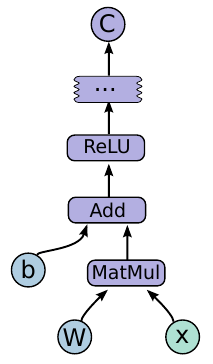
\includegraphics[scale=.685]{img/computation.png}
				\caption{Esempio di Grafo di Computazione, corrispondente alla Figura \ref{py:tfcode}}
				\label{fig:computation}
			\end{figure}
				
		
		\section{Implementazione}
			Le componenti principali del sistema TensorFlow sono il \textit{client} e il \textit{master}. Il client usa le sessioni per comunicare con il master. Vengono usati uno o più \textit{worker process} per accedere a uno o più \textit{device} con capacità di calcolo. L'interfaccia di TensorFlow è stata implementata sia per ambiente locale che distribuito.
			\begin{description}
				\item[Locale] Client, master e worker si trovano sulla stessa macchina nel contesto di un singolo processo di sistema operativo.
				\item[Distribuito] Client, master e worker si trovano in diversi processi potenzialmente su macchine fisiche diverse.
			\end{description}
			Ogni worker è responsabile di uno o più \textit{device} (Figura \ref{py:device}), e ogni device ha il suo tipo e nome. Nello scenario del singolo device è abbastanza facile eseguire il grafo: le dipendenze fra nodi sono facilmente individuabili e l'esecuzione dei nodi viene gestita tramite una pila, secondo una politica non meglio specificata. Discorso diverso per device multipli, e quindi anche per l'ambiente distribuito.
			\begin{figure*}
				\centering
				\begin{python}
with tf.Session() as sessione:
	with tf.device("/gpu:1"):
		matrice1 = tf.constant([[3., 3.]])
		matrice2 = tf.constant([[2.],[2.]])
		prodotto = tf.matmul(matrice1, matrice2)
				\end{python}
				\caption{Vincolo di esecuzione tramite la \texttt{GPU 1} presente nel sistema}
				\label{py:device}
			\end{figure*}
			\subsection{Esecuzione su device multipli}
				Per gestire la presenza di device multipli vengono adottati nuovi accorgimenti, è infatti necessario saper decidere a quale device assegnare la computazione di un dato nodo e saper comunicare fra grafi o sottografi che si trovano in posti diversi.
				\paragraph*{Posizionamento dei nodi} Una delle prime preoccupazioni di TensorFlow è quella di mappare i nodi all'insieme dei device disponibili, e viene fatto tramite un apposito \textbf{algoritmo di posizionamento}. In base ad alcune euristiche, a tempo statico viene approssimato l'input di tale algoritmo, e viene detto \textbf{modello di costo}. Per ogni nodi esso contiene la stima dei suoi tensori in input e in output espressa in byte e la stima del tempo di esecuzione. Ora che possiede l'input, l'algoritmo di posizionamento lancia un'esecuzione simulata del grafo, dove in base a euristiche \textit{greedy} è in grado di scegliere l'opportuno device.
				\paragraph{Comunicazione tra Device} A questo punto ogni device all'interno del sistema ha un proprio sottografo da eseguire. Ogni arco che unisce sottografi diversi e che quindi va dal nodo $x$ a $y$, viene sostituito con un arco che va da $x$ a \textit{send} e un'altro che va da \textit{recv} a $y$. \textit{send} e \textit{recv} sono nuovi nodi introdotti che gestiscono tutti i messaggi entranti e uscenti da un sottografo. Un po' come il corriere che si occupa di raccogliere tutte le spedizioni di una giornata, le porta in un'altro stato e le distribuisce ai relativi destinatari. Questo approccio permette di trasmettere dati una sola volta; permette che la memoria che spetta a un tensor sia allocata una sola volta anzi che più, e che nonostante il posizionamento dei nodi, l'utente possa esplicitamente assegnare l'esecuzione di un nodo a un determinato device (Figura \ref{py:device}).
			\subsection{Esecuzione Distribuita}
				L'approccio adottato per l'esecuzione distribuita di un grafo è quasi identico a quello preservato per i device. Qui la comunicazione tra grafi avviene tramite protocollo \texttt{TCP} o \texttt{RDMA}. Un'altra differenza è che negli ambienti distribuiti urge riflettere a una gestione degli errori di comunicazione. Gli errori possono avvenire tra i nodi \textit{send} e \textit{recv}, quindi è necessario verificare la salute degli scambi fra questi. Quando un fallimento viene rilevato l'esecuzione dell'intero grafo viene riavviata, ma questo non implica la perdita dei dati: si ricordi che i nodi variabile immagazzinano i tensors. Periodicamente vengono creati dei check-point dato che i nodi variabili sono collegati a speciali \textit{save node}, quindi è possibile ricoverare stati di esecuzione precedenti.
		\section{Estensioni}
			Essendo TensorFlow dedicato all'apprendimento automatico, il basilare modello di programmazione comprende alcuni strumenti specializzati. 
			
		\section{Ottimizzazioni}
			Poca attenzione
			
		\section{Parallelismo}
		
		\section{Strumenti}
		
		\section{Appunti Bart}		
		
		\begin{thebibliography}{9}
			\bibitem{tf}
			Google Research,
			\emph{TensorFlow: Large-Scale Machine Learning on Heterogeneous Distributed Systems},
			Preliminary White Paper,
			2015.
		\end{thebibliography}
	\end{multicols}

\end{document}